\documentclass[11pt,a4paper,openany]{book}
\usepackage[margin=24mm]{geometry}
\usepackage{fontspec}
\IfFontExistsTF{Noto Serif}{\setmainfont{Noto Serif}}{\setmainfont{DejaVu Serif}}
\usepackage{amsmath,amssymb,tikz,enumitem,microtype}
\usepackage[hidelinks]{hyperref}
\setlength{\parindent}{0pt}
\setlength{\parskip}{6pt}
\setlist[enumerate]{leftmargin=*,itemsep=8pt}
\setlength{\emergencystretch}{2em}

\renewcommand{\contentsname}{Contents}
\begin{document}
\title{V-TALENT 2045\\ PHY201-A --- Vectors, calculus and approximation for physics\\\large Level 2 \textbar{} Mathematics for Physics}
\author{Dr. Dang Minh Tuan -- TS. Đặng Minh Tuấn}
\date{2026 \textbar{} Draft v1.0}
\maketitle
\tableofcontents
\chapter*{How to study}
Grades 10–12 / Olympiad bridge. Prerequisites: algebra, trigonometry, coordinate geometry and PHY101-A concepts. Calculus is developed from physical meaning; ODE and complex numbers continue in PHY201-B.

Read the objective and answer the diagnostic before theory. Reproduce the worked solutions without looking, solve the exercises independently, then use the full solutions at the end to diagnose errors. Use a separate notebook for predictions, diagrams and checks. Original teaching text and exercises; external sources are reading locators, not reproduced. Draft pending independent review.
\chapter{Vectors, projections and physical products}
\section{Objectives and diagnostic}
Resolve vectors, use dot and cross products with units, and identify geometric constraints.

\textbf{Predict:} Can a nonzero force do zero work? Can a nonzero force exert zero torque?
\section{Theory and derivations}
A vector is not a list of numbers alone: components depend on the basis. In an orthonormal Cartesian frame, $\vec a=a_x\hat e_x+a_y\hat e_y+a_z\hat e_z$, and $|\vec a|=\sqrt{a_x^2+a_y^2+a_z^2}$. A unit vector $\hat n$ has magnitude one. The scalar projection $\vec a\cdot\hat n$ is signed, while the vector projection is $(\vec a\cdot\hat n)\hat n$. The perpendicular remainder is $\vec a-(\vec a\cdot\hat n)\hat n$. This decomposition is the basis of free-body diagrams, component kinematics and field measurements.

The dot product satisfies $\vec a\cdot\vec b=a_xb_x+a_yb_y+a_zb_z=ab\cos\theta$. Derive the geometric form by expanding $|\vec a-\vec b|^2$ and comparing with the cosine rule. Work by a constant force is $W=\vec F\cdot\Delta\vec r$; instantaneous power is $P=\vec F\cdot\vec v$. Both are scalars with signs. A force perpendicular to displacement does no work, though it can change the direction of velocity.

In a right-handed basis, $\vec a\times\vec b=(a_yb_z-a_zb_y,\ a_zb_x-a_xb_z,\ a_xb_y-a_yb_x)$. Its magnitude is $ab\sin\theta$ and direction follows the right-hand rule. It is antisymmetric: $\vec b\times\vec a=-\vec a\times\vec b$. Torque about a specified origin is $\vec\tau=\vec r\times\vec F$; magnetic force is $\vec F=q\vec v\times\vec B$. The torque depends on the choice of origin. The magnetic force is perpendicular to velocity and does not change kinetic energy by itself in classical mechanics.

For a vector equation, project onto independent directions to get scalar equations. Choosing axes along a plane or a constraint often simplifies the model. In three dimensions, a torque component about unit axis $\hat n$ is $\tau_n=(\vec r\times\vec F)\cdot\hat n$. Do not confuse the magnitude of total torque with a component about a particular hinge.
\begin{center}
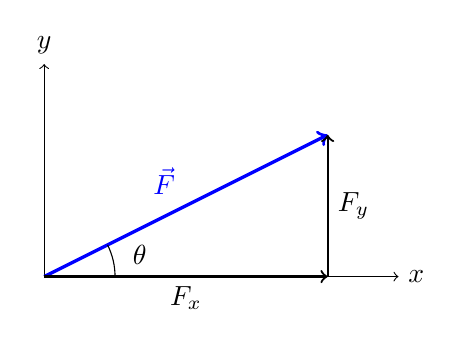
\begin{tikzpicture}[scale=.9]\draw[->](0,0)--(5,0)node[right]{$x$};\draw[->](0,0)--(0,3)node[above]{$y$};\draw[->,very thick,blue](0,0)--node[above left]{$\vec F$}(4,2);\draw[dashed](4,2)--(4,0);\draw[->,thick](0,0)--node[below]{$F_x$}(4,0);\draw[->,thick](4,0)--node[right]{$F_y$}(4,2);\draw (1,0) arc(0:26.565:1);\node at (1.35,.3){$\theta$};\end{tikzpicture}
\end{center}
\section{Worked examples}
\subsection*{Example 1.1}
A force F=(3,-4,2) N moves a particle by d=(2,1,-1) m. Find work and the angle between vectors.

\textbf{Solution.} $W=6-4-2=0$ J. Both vectors are nonzero, so $\cos\theta=0$ and $\theta=90^\circ$. A nonzero force can do zero work over the displacement.
\subsection*{Example 1.2}
A force (0,5,0) N acts at r=(0.3,0,0.4) m. Compute torque and its z-component.

\textbf{Solution.} $\vec\tau=(-2,0,1.5)$ N m; $\tau_z=1.5$ N m. Magnitude $\sqrt{4+2.25}=2.5$ N m. The hinge about z responds to the z-component, not total magnitude.
\subsection*{Example 1.3}
Resolve gravity into components along and normal to a frictionless 30\textdegree{} slope for a 2 kg block (g=9.81).

\textbf{Solution.} Downslope component $mg\sin30^\circ=9.81$ N; into-surface component $mg\cos30^\circ\approx16.99$ N. Normal reaction is 16.99 N if there is no normal acceleration or other normal force.
\section{Investigation}
Use a light ruler pivoted near one end and small known weights. Predict torque as a function of the perpendicular lever arm; compare balanced configurations. Keep the pivot fixed and avoid heavy loads.
\section{Modern application and transfer}
A robot joint at the origin experiences a load at $\vec r=(0.4,0.2,0)$ m with force $\vec F=(0,-30,0)$ N. The torque is $(0,0,-12)$ N m. A motor must counter this static moment, plus other loads. Transfer: compare changing the perpendicular moment arm with changing the force direction; identify why the same force can require very different actuator torque.
\section{Source-guided reading}
SW-1.1.1 and SW-1.1.2: pp. 13–18; SJ-05: ch. 5, pp. 20–24; SJ-17: torque and angular momentum, pp. 68–73.
\section{Independent practice}
\begin{enumerate}
\item \textbf{PHY201-A-1.1}. Find the projection of a=(4,3,0) onto unit vector n=(3/5,4/5,0).
\item \textbf{PHY201-A-1.2}. Find a\ensuremath{\times}b for a=(1,2,3), b=(0,1,-1), then verify perpendicularity.
\item \textbf{PHY201-A-1.3}. A force (5,-2,0) N acts while velocity is (-1,4,0) m/s. Determine instantaneous power and interpret its sign.
\item \textbf{PHY201-A-1.4}. A positive charge 2 \ensuremath{\mu}C moves at (3000,0,0) m/s in B=(0,0,0.2) T. Find magnetic force.
\item \textbf{PHY201-A-1.5}. For r=(0.2,0.3,0) m and F=(10,0,0) N, find torque about the origin and about point O\ensuremath{\prime}=(0,0.3,0).
\end{enumerate}
\chapter{Differentiation: rates, extrema and local models}
\section{Objectives and diagnostic}
Derive velocity and acceleration, apply chain/product rules and test extrema against domain boundaries.

\textbf{Predict:} At maximum displacement in SHM, what are velocity and acceleration?
\section{Theory and derivations}
The derivative $f'(x)=\lim_{h\to0}[f(x+h)-f(x)]/h$ describes the local linear response when the limit exists. Its units are those of $f$ divided by those of $x$. For $x(t)$, $v=dx/dt$, $a=d^2x/dt^2$. Starting from the limit for $t^2$, the quotient is $2t+h$, hence derivative $2t$. A zero velocity at an instant does not imply zero acceleration.

The product rule is $(fg)'=f'g+fg'$; chain rule is $d f(g(t))/dt=f'(g(t))g'(t)$. For $x=A\cos(\omega t+\phi)$, $v=-A\omega\sin(\omega t+\phi)$ and $a=-\omega^2x$. Angles in derivative formulas for trigonometric functions are in radians. For fixed mass, $d(mv^2/2)/dt=mv\,dv/dt=Fv$ in one dimension; this links energy and force.

For a differentiable function at an interior extremum, $f'=0$ is necessary, not sufficient. If $f''>0$ there is a local minimum; if $f''<0$ a local maximum; if $f''=0$ the test is inconclusive. Also evaluate endpoints, nonsmooth points and constraints. In a conservative one-dimensional system, $F=-dU/dx$; equilibrium has $U'=0$. A strict local minimum of $U$ yields stable equilibrium in the usual conservative setting, with $U''>0$ sufficient for a quadratic minimum.

For experimental data, a central difference $[x(t+h)-x(t-h)]/(2h)$ estimates velocity. Reducing $h$ reduces smooth-function truncation error but can amplify measurement noise. Numerical derivatives require a justified time step and uncertainty analysis. SIM-M02 compares the exact derivative with a finite difference for a cubic trajectory.
\begin{center}
\begin{tikzpicture}[x=.8cm,y=.48cm]\draw[->](0,0)--(5,0)node[right]{$t$};\draw[->](0,0)--(0,17)node[above]{$x$};\draw[blue,thick,domain=0:4,samples=60]plot(\x,{\x*\x});\draw[orange,thick](1,0)--(4,12);\fill(2,4)circle(2pt);\node[right]at(3,9){$x=t^2$};\node[right]at(4,12){$v(2)=4$};\end{tikzpicture}
\end{center}
\section{Worked examples}
\subsection*{Example 2.1}
For x(t)=2t\textsuperscript{3}-3t\textsuperscript{2}+4 (SI), find velocity and acceleration at t=2 s.

\textbf{Solution.} $v=6t^2-6t$, $a=12t-6$. Thus $v(2)=12$ m/s and $a(2)=18$ m/s$^2$. Coefficients implicitly carry units.
\subsection*{Example 2.2}
For x=0.08 cos(5t), find maximum speed and acceleration at x=+0.08 m.

\textbf{Solution.} $v=-0.4\sin5t$, so $|v|_{\max}=0.4$ m/s. $a=-25x$; at $x=0.08$, $a=-2$ m/s$^2$. Velocity is zero there.
\subsection*{Example 2.3}
For U(x)=x⁴-4x\textsuperscript{2} (in consistent units), locate and classify equilibria.

\textbf{Solution.} $U'=4x^3-8x=4x(x^2-2)$; equilibria $x=0,\pm\sqrt2$. $U''=12x^2-8$ equals -8 at 0 (unstable maximum) and 16 at $\pm\sqrt2$ (stable minima).
\section{Investigation}
Use SIM-M02, compute finite differences at t=2 for h=0.5, 0.2 and 0.1 s, then add a hypothetical position error of \ensuremath{\pm}0.01 m to the two endpoints. Compare truncation error with worst-case measurement error.
\section{Modern application and transfer}
A chip's simplified temperature response after switch-on is $T(t)=T_a+\Delta T(1-e^{-t/\tau})$. Its heating rate is $dT/dt=(\Delta T/\tau)e^{-t/\tau}$. For $\Delta T=40$ K and $\tau=20$ s, initial rate is 2 K/s; at 20 s it is $2/e\approx0.736$ K/s. Transfer: estimate the time constant from the time to reach 63.2 percent of the final temperature rise. Explain why a multi-component chip may not follow a single exponential.
\section{Source-guided reading}
SW-1.2.1–1.2.5: pp. 19–30; SJ-02: pp. 10–12; SJ-04: pp. 14–19.
\section{Independent practice}
\begin{enumerate}
\item \textbf{PHY201-A-2.1}. Differentiate x=4t-t\textsuperscript{2} and identify the turning time and acceleration.
\item \textbf{PHY201-A-2.2}. For v=6e^(-t/3) m/s, find a(0) and a(3 s).
\item \textbf{PHY201-A-2.3}. A constant mass 2 kg has v=3t\textsuperscript{2}. Find kinetic energy and its rate at t=2 s.
\item \textbf{PHY201-A-2.4}. Maximize P=12I-2I\textsuperscript{2} over 0\ensuremath{\le}I\ensuremath{\le}4 A. Compare endpoints.
\item \textbf{PHY201-A-2.5}. For x=t\textsuperscript{3}, derive the central-difference estimate at t for step h and its error.
\end{enumerate}
\chapter{Integration, accumulation and initial conditions}
\section{Objectives and diagnostic}
Derive accumulated change and work, use definite integrals, integrate densities and validate units.

\textbf{Predict:} When the integral of velocity is zero, has an object necessarily remained at rest?
\section{Theory and derivations}
An integral sums local contributions: partition an interval into small widths $\Delta x_i$ and approximate $\sum f(x_i)\Delta x_i$. In the limit the definite integral is $\int_a^b f(x)\,dx$. Signed area is not always geometric area. For a continuous velocity, displacement is $\int_{t_0}^{t_1}v(t)\,dt$ and distance is $\int_{t_0}^{t_1}|v(t)|\,dt$. The fundamental theorem connects a rate to its accumulated change: $F'=f$ implies $\int_a^b f(x)\,dx=F(b)-F(a)$.

From $a(t)=dv/dt$, $v(t)=v_0+\int_{t_0}^t a(s)\,ds$ and $x(t)=x_0+\int_{t_0}^t v(s)\,ds$. The initial conditions determine integration constants. In one dimension work by a variable force is $W=\int_{x_a}^{x_b}F(x)\,dx$; for a path in space it generalises to $\int\vec F\cdot d\vec r$. When $F$ is conservative, $U(b)-U(a)=-W$. For ideal spring force $F=-kx$, integrating gives $U(x)-U(0)=kx^2/2$.

Substitution changes variables, for example $\int 2t e^{-t^2}dt=-e^{-t^2}+C$. Integration by parts follows from the product rule: $\int u\,dv=uv-\int v\,du$. For distributed bodies, $dm=\lambda(x)dx$ and $m=\int dm$; center of mass $x_{\rm cm}=\int x\,dm/m$. The moment of inertia about a chosen axis is $I=\int r_\perp^2\,dm$. Integrate with respect to the appropriate geometry; $r_\perp$ is distance to the axis, not necessarily distance to the origin.
\begin{center}
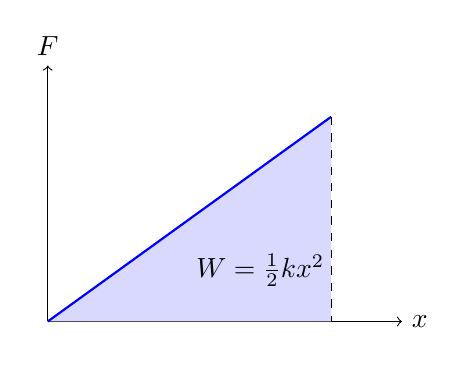
\begin{tikzpicture}[x=.9cm,y=.65cm]\draw[->](0,0)--(5,0)node[right]{$x$};\draw[->](0,0)--(0,5)node[above]{$F$};\fill[blue!15](0,0)--(4,4)--(4,0)--cycle;\draw[thick,blue](0,0)--(4,4);\draw[dashed](4,4)--(4,0);\node at (3,1){$W=\frac12kx^2$};\end{tikzpicture}
\end{center}
\section{Worked examples}
\subsection*{Example 3.1}
Acceleration a=2t, initial v=3 m/s and x=1 m. Find v(t), x(t) and x(2).

\textbf{Solution.} $v=3+\int_0^t2s\,ds=3+t^2$. $x=1+\int_0^t(3+s^2)\,ds=1+3t+t^3/3$. At 2 s, $x=1+6+8/3=29/3$ m.
\subsection*{Example 3.2}
A force F(x)=4x+3 N acts along x from 0 to 2 m. Find work and average force over distance.

\textbf{Solution.} $W=\int_0^2(4x+3)dx=[2x^2+3x]_0^2=14$ J. Distance-weighted mean force $W/2=7$ N.
\subsection*{Example 3.3}
A rod extends from x=0 to L with linear density \ensuremath{\lambda}(x)=\ensuremath{\lambda}\textsubscript{0}x/L. Find total mass and center of mass.

\textbf{Solution.} $m=(\lambda_0/L)\int_0^L x\,dx=\lambda_0L/2$. First moment $(\lambda_0/L)\int_0^Lx^2dx=\lambda_0L^2/3$. Hence $x_{\rm cm}=2L/3$, toward the denser end.
\section{Investigation}
Approximate work for F=4x+3 on 0\ensuremath{\le}x\ensuremath{\le}2 using left and right rectangles with 4, 8 and 16 intervals. Compare with 14 J and explain why the two sums bracket the exact value for this increasing force.
\section{Modern application and transfer}
An electric sensor draws $I(t)=0.1e^{-t/5}$ A from a regulated 3 V supply for 10 s. Charge used is $Q=\int_0^{10}I(t)dt=0.5(1-e^{-2})\approx0.432$ C. Energy supplied is $E=3Q\approx1.30$ J. Transfer: if the supply voltage varies, energy must be calculated as $\int U(t)I(t)dt$, not as the product of independent time averages.
\section{Source-guided reading}
SW-1.3.1–1.3.5: pp. 35–49; SJ-03: pp. 12–14; SJ-20: pp. 86–89; JP-A: mathematical physics appendix.
\section{Independent practice}
\begin{enumerate}
\item \textbf{PHY201-A-3.1}. Integrate v=4-2t over 0\ensuremath{\le}t\ensuremath{\le}4. Determine displacement and distance.
\item \textbf{PHY201-A-3.2}. For spring constant 80 N/m, compute work by the spring from x=0.1 to 0.3 m.
\item \textbf{PHY201-A-3.3}. A uniform thin rod of length L and mass m rotates about an axis perpendicular to the rod through one end. Derive I.
\item \textbf{PHY201-A-3.4}. Evaluate \ensuremath{\int}\textsubscript{0}¹ 2x/(1+x\textsuperscript{2}) dx and state the substitution.
\item \textbf{PHY201-A-3.5}. For F(x)=kx\textsuperscript{2} with k>0, derive work from 0 to L and the unit of k.
\end{enumerate}
\chapter{Taylor approximation, dimensional analysis and polar coordinates}
\section{Objectives and diagnostic}
Use dimensionless small parameters, justify approximation errors, derive polar velocity and acceleration.

\textbf{Predict:} Why is the small-angle approximation meaningful only after specifying radians?
\section{Theory and derivations}
Taylor expansion about $x_0$ is $f(x_0+h)=f(x_0)+hf'(x_0)+h^2f''(x_0)/2+\cdots$ when the relevant smoothness and convergence conditions hold. The first-order approximation is local. For a small dimensionless parameter $\epsilon$, $(1+\epsilon)^n\approx1+n\epsilon$; the next term is $n(n-1)\epsilon^2/2$. In radians, $\sin\theta\approx\theta$ and $\cos\theta\approx1-\theta^2/2$. For real $\theta$, the sine first-order absolute error is bounded by $|\theta|^3/6$. Choose a tolerance before deciding to truncate.

Dimensional analysis can constrain exponents. Suppose the period of a simple pendulum depends only on length $l$ and gravitational acceleration $g$: $T=C l^a g^b$. Matching time exponent gives $-2b=1$, so $b=-1/2$; length exponent gives $a+b=0$, hence $a=1/2$. Thus $T=C\sqrt{l/g}$. The small-angle dynamics gives $C=2\pi$; dimensions alone cannot determine it or rule out dependence on dimensionless amplitude. A model's chosen variables must be physically justified.

In planar polar coordinates $\vec r=r\hat e_r$, where $\hat e_r=(\cos\theta,\sin\theta)$ and $\hat e_\theta=(-\sin\theta,\cos\theta)$. Differentiation yields $\dot{\hat e}_r=\dot\theta\hat e_\theta$, $\dot{\hat e}_\theta=-\dot\theta\hat e_r$. Hence $\vec v=\dot r\hat e_r+r\dot\theta\hat e_\theta$ and $\vec a=(\ddot r-r\dot\theta^2)\hat e_r+(r\ddot\theta+2\dot r\dot\theta)\hat e_\theta$. These terms arise from the changing basis; omitting basis derivatives loses centripetal and cross terms. Uniform circular motion has $\dot r=\ddot r=\ddot\theta=0$ and $a_r=-r\omega^2$.

For field and volume integrals, a polar area element is $dA=r\,dr\,d\theta$; cylindrical volume $dV=r\,dr\,d\theta\,dz$; spherical volume $dV=r^2\sin\theta\,dr\,d\theta\,d\phi$ where $\theta$ is the polar angle. These factors describe geometric stretching of coordinate cells. For example $\int_0^{2\pi}\int_0^R r\,dr\,d\theta=\pi R^2$. Full vector calculus is a later extension.
\begin{center}
\begin{tikzpicture}[scale=.85]\draw[->](0,0)--(5,0)node[right]{$x$};\draw[->](0,0)--(0,4)node[above]{$y$};\draw[gray](0,0)circle(2.5);\draw[->,thick](0,0)--(2,1.5)node[midway,above left]{$r$};\draw[->,blue,very thick](2,1.5)--(3.2,2.4)node[right]{$\hat e_r$};\draw[->,orange,very thick](2,1.5)--(1.1,2.7)node[above]{$\hat e_\theta$};\draw(.9,0)arc(0:36.87:.9);\node at(1.2,.35){$\theta$};\end{tikzpicture}
\end{center}
\section{Worked examples}
\subsection*{Example 4.1}
For \ensuremath{\theta}=0.2 rad, estimate sin \ensuremath{\theta} using first and third order; bound first-order absolute error.

\textbf{Solution.} First order 0.2. Third order $0.2-0.2^3/6=0.1986667$. Bound $0.2^3/6=0.0013333$. Actual $\sin0.2\approx0.1986693$, consistent.
\subsection*{Example 4.2}
Assume wave speed depends only on fluid pressure p and density \ensuremath{\rho}. Derive a dimensional form.

\textbf{Solution.} $v=Cp^a\rho^b$. Dimensions: $ML^{-1}T^{-2}$ and $ML^{-3}$. Matching gives $a+b=0$, $-2a=-1$, $-a-3b=1$. Thus $a=1/2,b=-1/2$ and $v=C\sqrt{p/\rho}$. In an ideal gas the adiabatic sound model gives $C=\sqrt\gamma$.
\subsection*{Example 4.3}
A particle has r=2+t (m) and \ensuremath{\theta}=3t (rad). Find polar velocity and acceleration components at t=1 s.

\textbf{Solution.} At t=1, $r=3$, $\dot r=1$, $\ddot r=0$, $\dot\theta=3$, $\ddot\theta=0$. Thus $(v_r,v_\theta)=(1,9)$ m/s and $(a_r,a_\theta)=(-27,6)$ m/s$^2$.
\section{Investigation}
Measure pendulum periods at approximate amplitudes 5\textdegree{}, 15\textdegree{} and 30\textdegree{} using a light bob and low amplitude. Compare with the small-angle period; discuss timing uncertainty and why a failure to detect a difference is not proof of amplitude independence.
\section{Modern application and transfer}
Near the bottom of a smooth potential well, $U(x)\approx U(0)+kx^2/2$ when $U'(0)=0$ and $k=U''(0)>0$. The force becomes $F\approx-kx$; therefore small displacements obey harmonic motion. This local approximation is central to lattice vibrations and resonant sensors. Transfer: for $U=U_0+kx^2/2+\beta x^4/4$, compare nonlinear and linear force magnitudes at amplitude A. Their ratio is $|\beta|A^2/k$; if this is not small, the harmonic model is inadequate.
\section{Source-guided reading}
SW-1.2.6: pp. 31–32; SW-1.3.5: p. 49; JP-A: pp. 323–337; JP-1.5: p. 8; SJ-15: pp. 56–59; SJ-22: pp. 92–94.
\section{Independent practice}
\begin{enumerate}
\item \textbf{PHY201-A-4.1}. Estimate (1.04)^(1/2) to second order and compare with the first-order result.
\item \textbf{PHY201-A-4.2}. Use the bound \ensuremath{\theta}\textsuperscript{3}/6 to find a sufficient positive angle limit for absolute sine approximation error \ensuremath{\le}0.001.
\item \textbf{PHY201-A-4.3}. Assume drag force depends only on density \ensuremath{\rho}, speed v and area A. Determine a monomial dimensionally.
\item \textbf{PHY201-A-4.4}. For r=0.5 m and \ensuremath{\theta}=4t, find speed and acceleration magnitude.
\item \textbf{PHY201-A-4.5}. Derive the area of an annulus with inner radius a and outer radius b using a polar integral.
\end{enumerate}
\chapter*{References and simulations}
Swiss Physics Olympiad Script, 3rd ed. (2019).\par
The Committee of Japan Physics Olympiad (2014). \textit{Physics Olympiad: Basic to Advanced Exercises}. World Scientific.\par
Tan Chien Hao (2024). \textit{Freshman Physics}.\par
\url{https://diavn.github.io/truongchuyen/physics-curriculum.html}\par
\url{https://diavn.github.io/truongchuyen/physics-math-lab.html}
\appendix
\chapter{Full solutions to independent practice}
\section{Vectors, projections and physical products}
\begin{enumerate}
\item \textbf{PHY201-A-1.1}. Scalar $a\cdot n=24/5$; vector $(24/5)n=(72/25,96/25,0)$. The perpendicular remainder has zero dot product with n.
\item \textbf{PHY201-A-1.2}. $\vec a\times\vec b=(-5,1,1)$. Dot with a gives $-5+2+3=0$; dot with b gives $1-1=0$.
\item \textbf{PHY201-A-1.3}. $P=-5-8=-13$ W. This force removes mechanical energy at that instant (other forces may supply energy).
\item \textbf{PHY201-A-1.4}. $\vec v\times\vec B=(0,-600,0)$; multiply by $2\times10^{-6}$ C: $\vec F=(0,-1.2\times10^{-3},0)$ N. Dot with v is zero.
\item \textbf{PHY201-A-1.5}. About origin $\tau_z=0.2(0)-0.3(10)=-3$ N m. About O\ensuremath{\prime}, relative position $(0.2,0,0)$ is parallel to F, so torque is zero.
\end{enumerate}
\section{Differentiation: rates, extrema and local models}
\begin{enumerate}
\item \textbf{PHY201-A-2.1}. $v=4-2t=0$ at $t=2$ s; sign changes positive to negative. $a=-2$ m/s$^2$.
\item \textbf{PHY201-A-2.2}. $a=-2e^{-t/3}$ m/s$^2$; $a(0)=-2$, $a(3)=-2/e\approx-0.736$ m/s$^2$.
\item \textbf{PHY201-A-2.3}. $K=v^2=9t^4$ J, $K(2)=144$ J; $dK/dt=36t^3=288$ W at 2 s. Check $Fv=2(12)(12)=288$ W.
\item \textbf{PHY201-A-2.4}. $P'=12-4I=0$ at $I=3$ A, $P''=-4$. Values: $P(0)=0$, $P(3)=18$, $P(4)=16$ W. Maximum 18 W.
\item \textbf{PHY201-A-2.5}. $[(t+h)^3-(t-h)^3]/(2h)=3t^2+h^2$. Exact derivative $3t^2$; truncation error is $h^2$ in the chosen consistent units. Halving h reduces it by four.
\end{enumerate}
\section{Integration, accumulation and initial conditions}
\begin{enumerate}
\item \textbf{PHY201-A-3.1}. Zero at t=2. $\int_0^4(4-2t)dt=0$; positive area 4 m, negative signed area -4 m, distance 8 m.
\item \textbf{PHY201-A-3.2}. $W=\int_{0.1}^{0.3}-80x\,dx=-40(0.09-0.01)=-3.2$ J. Potential energy increases 3.2 J.
\item \textbf{PHY201-A-3.3}. $dm=(m/L)dx$. $I=(m/L)\int_0^L x^2dx=mL^2/3$.
\item \textbf{PHY201-A-3.4}. $u=1+x^2$, $du=2x\,dx$. Limits 1 and 2, integral $\int_1^2du/u=\ln2$.
\item \textbf{PHY201-A-3.5}. $W=kL^3/3$. Since $F$ is N and x\textsuperscript{2} is m\textsuperscript{2}, $[k]=$ N/m$^2$. Work units are N m.
\end{enumerate}
\section{Taylor approximation, dimensional analysis and polar coordinates}
\begin{enumerate}
\item \textbf{PHY201-A-4.1}. $\sqrt{1+\epsilon}\approx1+\epsilon/2-\epsilon^2/8$. At 0.04: first order 1.02; second 1.0198. Exact about 1.0198039.
\item \textbf{PHY201-A-4.2}. $\theta^3/6\le0.001$ requires $\theta\le(0.006)^{1/3}\approx0.1817$ rad, approximately $10.4^\circ$. This is sufficient, not claimed necessary.
\item \textbf{PHY201-A-4.3}. $F=C\rho^a v^b A^c$. Mass gives $a=1$, time gives $b=2$, length gives $-3+2+2c=1$ so $c=1$. Therefore $F=C\rho v^2 A$; actual coefficient depends on shape, Reynolds number and regime.
\item \textbf{PHY201-A-4.4}. $v=r\omega=2$ m/s; $a=r\omega^2=8$ m/s$^2$, inward.
\item \textbf{PHY201-A-4.5}. $A=\int_0^{2\pi}\int_a^b r\,dr\,d\theta=2\pi(b^2-a^2)/2=\pi(b^2-a^2)$. Limits agree for a=0 and a=b.
\end{enumerate}
\end{document}
